\subsection{Wire Lattice structure}

\begin{frame}{Wire Lattice structure}
    \begin{columns}
        \column{0.5\textwidth}
        \begin{itemize}
            \item Effective permittivity \cite{PhysRevLett.76.4773}:
        \end{itemize}
        \begin{equation*}
            \varepsilon (\omega) = \varepsilon_0 \left( 1 - \dfrac{\omega_{P \varepsilon}^2}{\omega^2 - j \gamma \omega } \right).
        \end{equation*}
        % \vspace{3mm}
        \begin{itemize}
            \item Plasma frequency
        \end{itemize}
        \begin{equation*}
            \omega_{P \varepsilon} = \sqrt{ \dfrac{2 \pi c_0^2}{a^2 \ln (a/R)} } \sim \dfrac{c_0}{a}.
        \end{equation*}
        \begin{itemize}
            \item Effective permittivity tensor:
        \end{itemize}
        \begin{equation*}
            \varepsilon_{eff} = \left(
            \begin{array}{ccc}
                \varepsilon_0 & 0 & 0 \\
                0 & \varepsilon_0 & 0 \\ 
                0 & 0 & \varepsilon (\omega)
            \end{array}
            \right) .
        \end{equation*}

        \column{0.5\textwidth}
        \vspace{-14mm}
        \begin{figure}
            \centering
            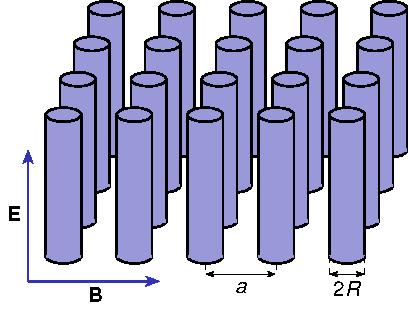
\includegraphics[width=0.8\textwidth]{Figures/Wire_lattice_structure.pdf}
            \caption{Wire lattice structure.}
            \label{fig:Wire_lattice_structure}
        \end{figure}
        \vspace{-8mm}
        \begin{figure}
            \centering
            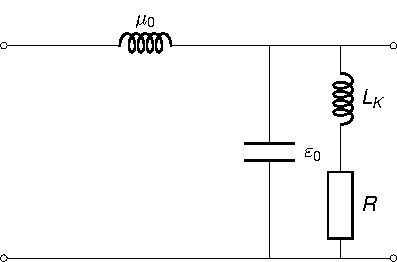
\includegraphics[width=0.8\textwidth]{Figures/TL_negative_permittivity.pdf}
            \caption{Equivalent circuit of wire lattice structure.}
            \label{fig:TL_negative_permittivity}
        \end{figure}
        
    \end{columns}
\end{frame}